
\chapter{Introduction : }
\section{Problématique : }
\paragraph{Limite de BSO }
Bien l'algorithme BSO (voir \ref{part2})présente des résultats très satisfaisants, il a cependant quelques points faibles qui sont liés à la recherche des bonnes valeurs des paramètres empiriques , l'ajustement dynamique a permit de palier a ce problème, mais il reste aussi l'aspect stochastique aléatoire très imprévisible des méta-heuristiques, c'est là qu'entre en scène une nouvelle familles de  M.H\footnote{Méta-heuristique} appelées ACO (\textbf{Ant Colony Optimization}) pour essayer de marier méthode constructive et méthode évolutionnaire.
\section{Définitions}
\subsection{Ant Colony Optimization(ACO)}
\paragraph{}
Les algorithmes de colonies de fourmis sont des algorithmes inspirés du comportement des fourmis, et qui constituent une famille de métaheuristiques d’optimisation principalement conçues pour des problèmes de \textbf{path-finding}\footnote{Problème visant a trouver le chemin le plus court d'un point de départ A à un point d'arrivée B}.
Dans cette partie du projet nous allons nous intéresser à deux implémentation d'une M.H ACO, à savoir \textbf{AS}(Ant System) et \textbf{ACS}(Ant Colony System).
\begin{figure}[H]
	\centering
	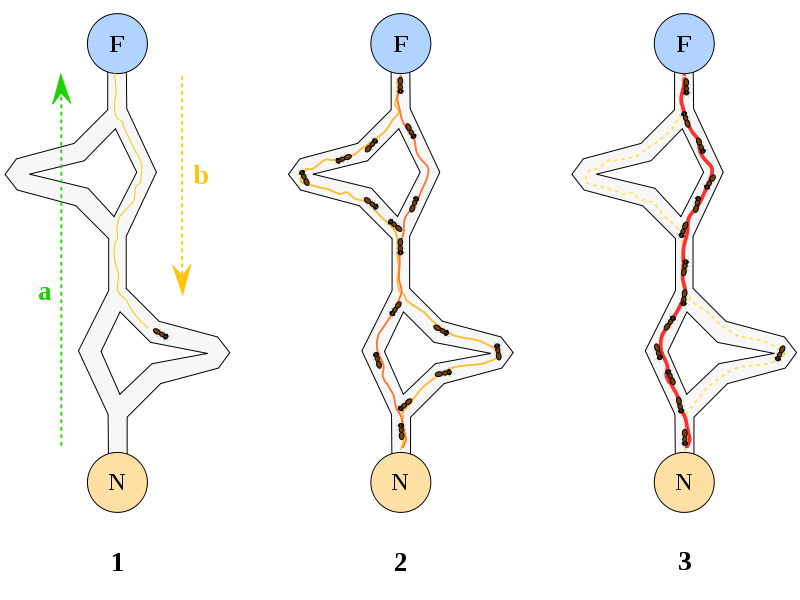
\includegraphics[scale=0.25]{images/ants.png}
	\caption{Abeilles communiquant pour la recherche de nourriture}
\end{figure}

\subsubsection{Ant System(AS)}
\paragraph{}\label{AS}
Cette variante d'ACO fut l'une des première a être développée, elle se base sur une approche probabiliste du choix du chemin a parcourir par la fourmille, en effet une fourmille en temps normal réagit à un stimulus naturel qui la \textbf{Phéromone}, une fourmille suivra instinctivement la trace de phéromones la plus forte la plus part du temps trace précédente.

\subsubsection{Ant Colony System(ACS)}
\paragraph{}\label{ACS}
Pensé comme une amélioration d'\textbf{AS}, ACS permet une modélisation plus fidèle à la vie réelle en introduisant les principes suivants: 
\begin{itemize}
	\item La mise a jour de la trace de phéromones enligne(effectuée par chaque fourmille lors de son passage sur un état) et hors-ligne(effectué à la fin de la construction de toutes les solutions des fourmilles)
	\item La marche aléatoire(RandomWalk\footnote{Modèle mathématique  d'un système possédant une évolution composée d'une succession de pas aléatoires, ou effectués « au hasard ».}) qui servira de règle de transition pour aller d'un état à un autre.
	\item Exploitation, c'est le fait de suivre la trace de phéromones la plus forte( le stimulus le plus fort).
	\item Exploration, c'est le fait de prendre l'initiative d'explorer de nouveaux états sans pour autant tenir compte de la trace de phéromones la plus forte
\end{itemize}


\subsection{Phéromones}
Pour finir il nous faut introduire le concept de la phéromone. Dans la nature, la phéromone es une molécule chimique produite par un organisme, qui induit un comportement spécifique chez un autre membre de la même espèce, dans notre cadre de la recherche de solutions optimales pour une problème donnée, elle peut être perçu comme une valeur numérique attaché un état de la solution(cela reste une interprétation générale qui peut varier selon le problème).



%Add it to implementation :
%, et déposera ensuite une petite quantité de cette phéromone sur son passage. quand toutes les fourmilles finissent de construire leur solution, une mise a jour des traces de phéromones est activée et cela selon la quantité déjà présente dans la